

\chapter{Chosen Plaintext Security}



\section{Reusing Keys}
	\begin{itemize}
	    \item Stream ciphers have shorter keys than the OTP
	    \item But still keys can only be used once
	    \item How can we make keys reusable?
	    \item First: How should this be modeled in the security definition?
	\end{itemize}
	
	
\section{Chosen Plaintext Attacks}
	\begin{itemize}
	    \item Key-Reuse: Adversary sees many encryptions under the same key
	    \item Not all of them might be unpredictable
	    \item Real Real world scenario: Adversary can influence what honest party encrypts
	    \item Conservative Approach: Let the adversary choose the messages of which he sees encryptions!
	    \item Idea: Give the adversary an \textbf{encryption oracle}
	\end{itemize}
	\begin{center}
		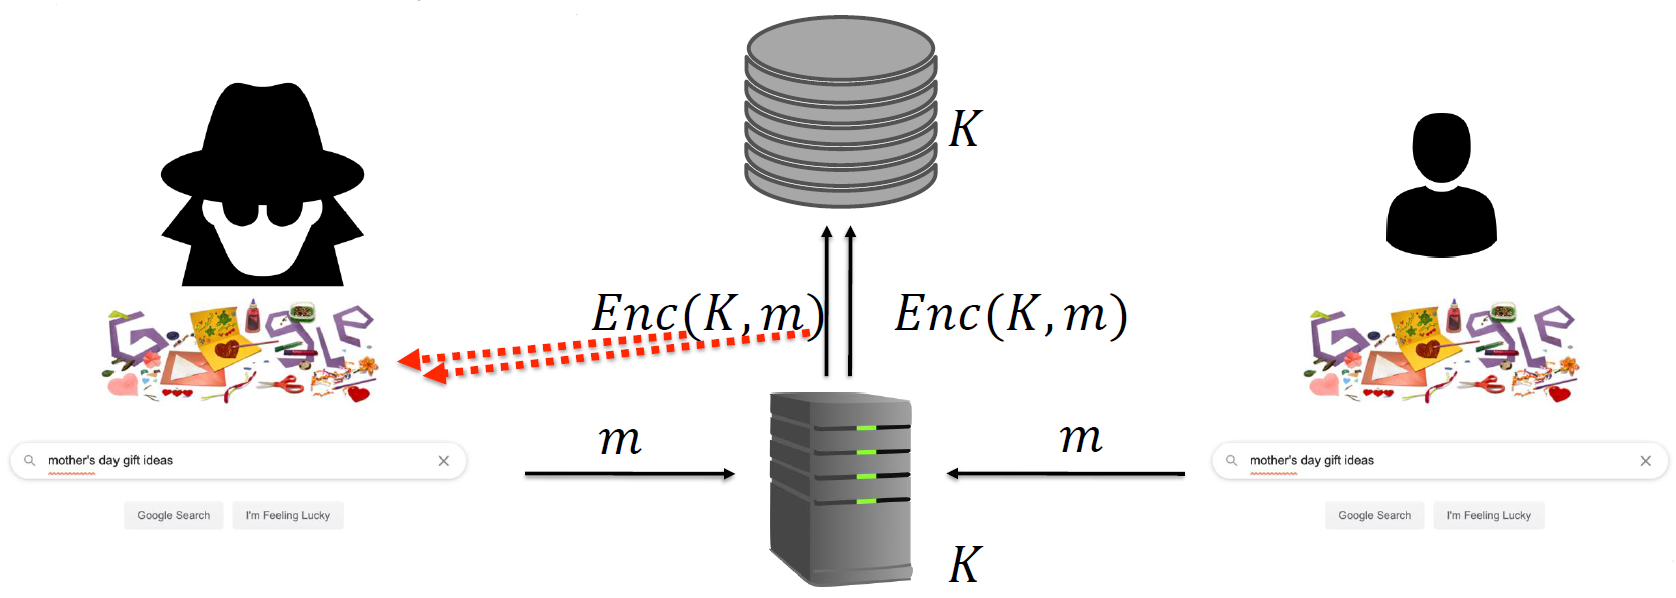
\includegraphics[width=160mm]{Graphics/CPA/cpa1.png}
	\end{center}
	
\newpage
	\begin{definition}[$IND-CPA$-secure]
	    An encryption scheme $(KeyGen,Enc,Dec)$ is $IND-CPA$-secure, if it hol;ds for every $PPT$-adversary $\mathcal{A}$ there exists a negligible function $v$ s.t. 
	    for all $\lambda \in \mathbb{N}$
	    $$Pr[IND-CPA_{\mathcal{A}}(\lambda)=1] < \frac{1}{2} + v(\lambda)$$
	    \begin{center}
			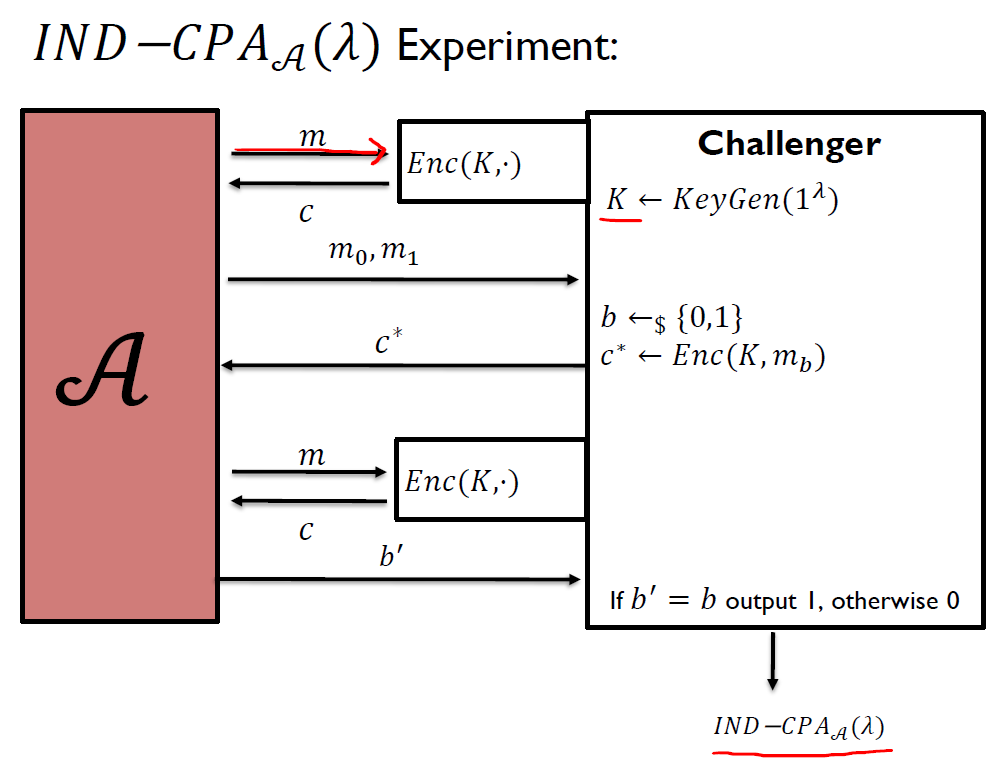
\includegraphics[width=120mm]{Graphics/CPA/cpa2.png}
		\end{center}
	\end{definition}
	
	
	
\section{Constructing IND-CPA secure encryption}
	\begin{itemize}
	    \item Observation: IND CPA secure encryption cannot be deterministic
	    \item Encryption needs to use randomness
	    \item To achieve this stronger security notion, we need stronger ingredient
	    \item PRGs: Small amount of randomness $\Rightarrow$ Larger amount of pseudorandomness
	    \item Needed: Small amount of randomness $\Rightarrow$ (Essentially) unlimited pseudorandomness
	\end{itemize}
	
	
	\begin{definition}[Pseudorandom Functions]\ 
	    \begin{itemize}
	        \item Efficiently computable keyed function (ensemble) $F_K: \{0,1\}^{\lambda} \to \{0,1\}^l$, where $K \in \{0,1\}^{\lambda}$
	        \item Uniformly random function $H: \{0,1\}^{\lambda} \to \{0,1\}^l$
	        \item I.e. for every $x \in \{0,1\}^{\lambda}$ it holds that $H(x)$ is independently uniformly random on $\{0,1\}^l$
	        \item $F$ is a pseudorandom function, if for every oracle PPT distinguisher $\mathcal{D}$ it holds
	        $$\vert Pr[\mathcal{D}^{F_K (\cdot)}(1^{\lambda})=1]-Pr[\mathcal{D}^{H (\cdot)}(1^{\lambda})=1] \vert < negl(\lambda)$$
	        where probability is over choice of $K \leftarrow_{\$} \{0,1\}^{\lambda}$, $H$ and random coins of $\mathcal{D}$.
	    \end{itemize}
	    \begin{center}
			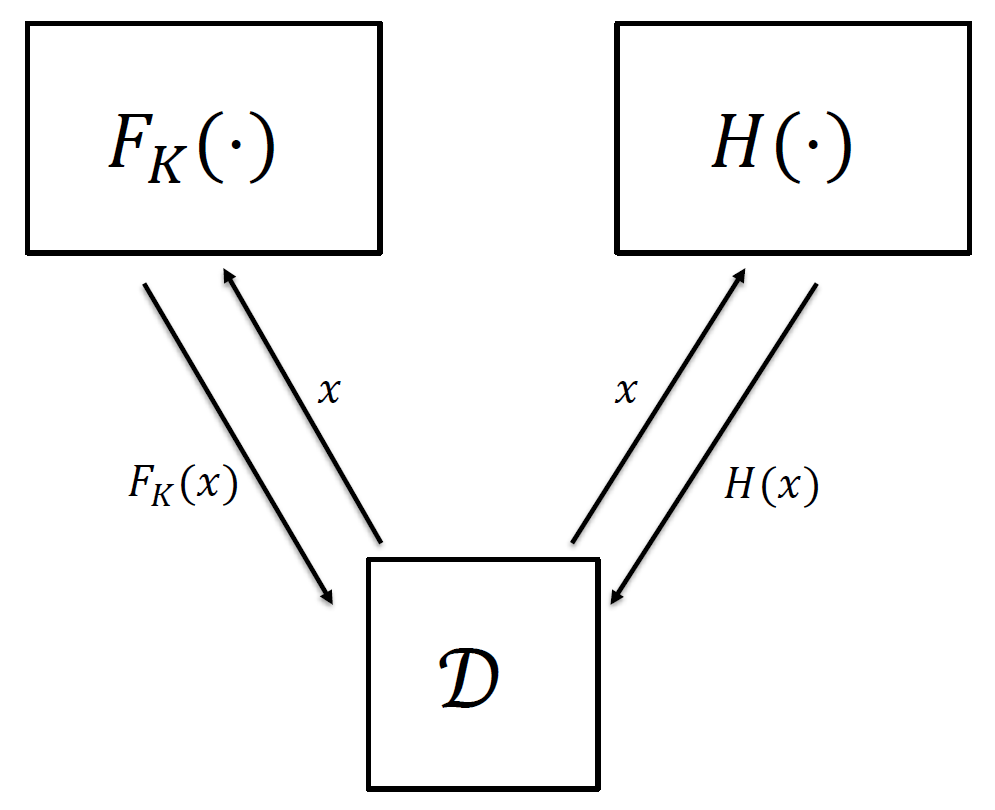
\includegraphics[width=120mm]{Graphics/CPA/prf.png}
		\end{center}
	\end{definition}
	
	
	\subsection{Examples}
		Assume $F, F'$ are PRFs:
		\begin{itemize}
			\item $F^*_{(K,K')}(x) = F_K(x) \oplus F'_{K'}(x)$\\
				$F^*_{(K,K')}(x)$ is a PRF, because
				$${\mathcal{D}^*}^{(F_K \oplus F'_{K'})(\cdot)} \approx {\mathcal{D}^*}^{(H \oplus F'_{K'})(\cdot)} \approx {\mathcal{D}^*}^{H'(\cdot)}$$
				with 
				$${\mathcal{D}^*}^{(F_K \oplus F'_{K'})(\cdot)} \text{ computes } F_K(x) \oplus F'_{K'}(x) \text{, and } 
				{\mathcal{D}^*}^{(H \oplus F'_{K'})(\cdot)} \text{ computes } H(x) \oplus F'_{K'}(x).$$
				Let $H(x)$ be an uniformly random function.\\
				If we XOR a function with an uniformly random function, the result is an uniformly random function too.
				So, $H'(x) := H(x) \oplus F'_{K'}(x)$ is an uniformly random function.\\
				(The proof of reduction was omitted)
			\item $F^*_K (x) = (F_K(x),F_K(x \oplus 1^n))$\\
				$F^*_K (x)$ is not a PRF, because
				$$F^*_K (x \oplus 1^n) = (F_K(x \oplus 1^n),F_K((x \oplus 1^n) \oplus 1^n)) = (F_K(x \oplus 1^n),F_K(x \oplus 1^n \oplus 1^n)) = (F_K(x \oplus 1^n),F_K(x))$$
				has the same output as $F^*_K(x)$ if we change the positions of the tupel.\\
				Therefore the outputs for the inputs $x$ and $x \oplus 1^n$ are correlated. 
		\end{itemize}
	
	
\section{Encryption from Pseudorandom Functions}
	\begin{center}
		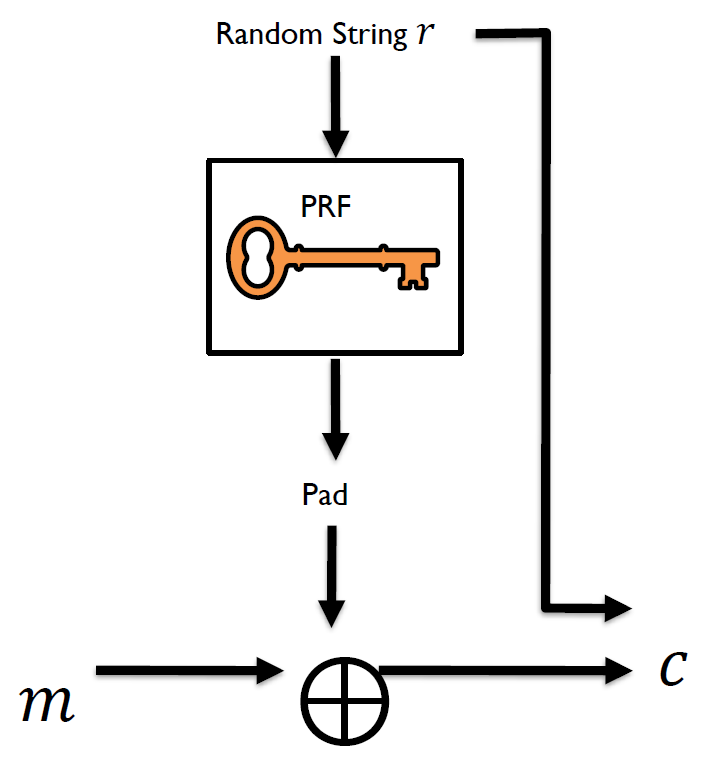
\includegraphics[width=48mm]{Graphics/CPA/cpa3.png}
	\end{center}
	\begin{itemize}
	    \item $KeyGen(1^{\lambda})$: Choose $K \leftarrow_{\$} \{0,1\}^{\lambda}$
	    \item $Enc(K,m)$: Choose $r \leftarrow_{\$} \{0,1\}^{\lambda}$, compute and output $c \leftarrow (r,F_K(r) \oplus m)$
	    \item $Dec(K,c)$: Parse $c=(r,y)$, compute and output $m \leftarrow F_K(r) \oplus y$
	    \item \textbf{Correctness:}
	    $$Dec(K,Enc(K,m))=Dec(K,(r,F_K(r) \oplus m))=F_K(r) \oplus F_K(r) \oplus m = m$$
	\end{itemize}
	
	
	\begin{theorem}[IND-CPA Security]\ 
		\begin{center}
			$F$ is a pseudorandom function $\Rightarrow$ $(KeyGen,Enc,Dec)$ is IND-CPA secure
		\end{center}
	\end{theorem}
	\begin{proof}
		Assume towards contradiction there exists a PPT $\mathcal{A}$ and a non-negligible $\epsilon$ so that
		$$Pr[IND-CPA_{\mathcal{A}}(\lambda) = 1] \geq \frac{1}{2} + \epsilon$$
		\underline{Show:}
		This implies distinguisher $\mathcal{D}$ against PRF $F$ with non-negligible advantage.\\
		First, a thought experiment. What if we use instead of an encryption scheme with a PRF
		$$Enc(K,m) = (r, F_K(r) \oplus m),$$
		a modified encryption scheme with an uniformly random function
		$$Enc'(m) = (r, H(r) \oplus m).$$
	    \begin{center}
			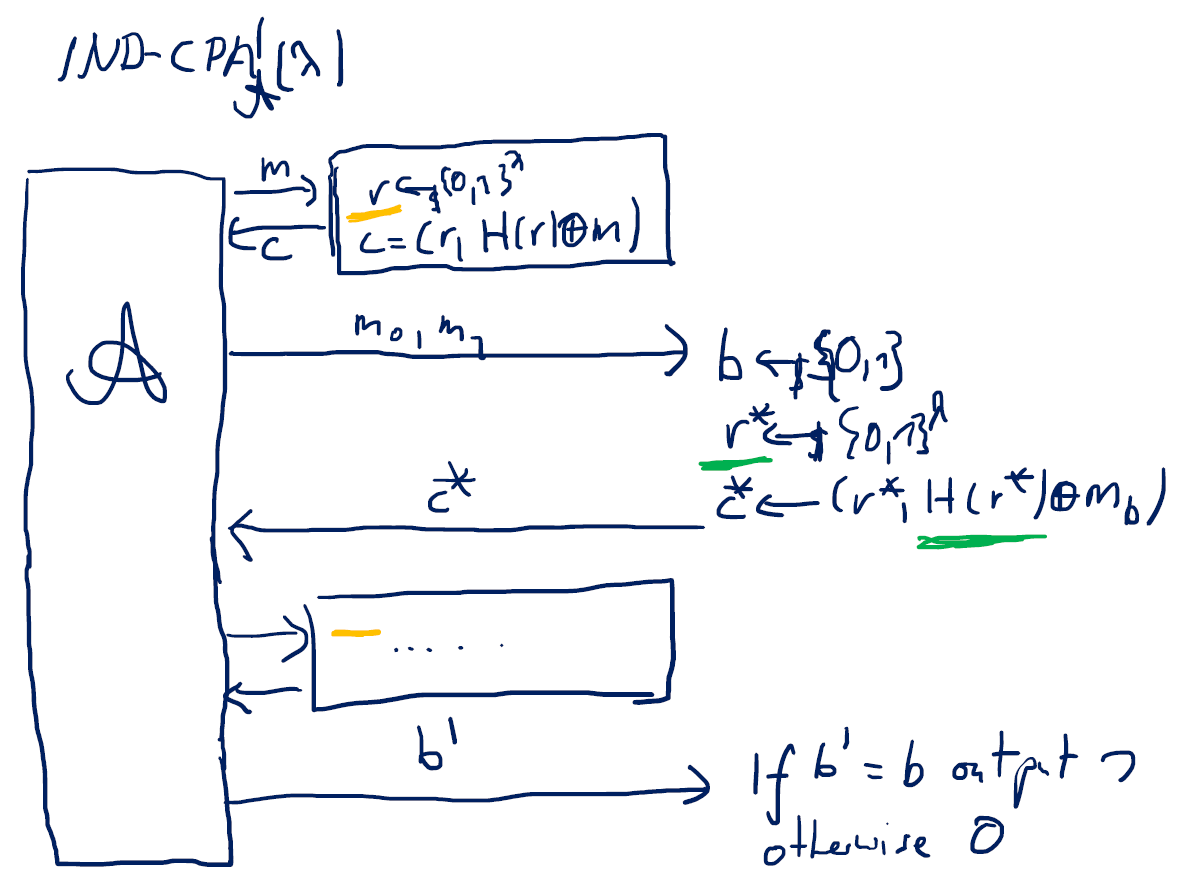
\includegraphics[width=110mm]{Graphics/CPA/cpa4.png}
		\end{center}
		How many r? $\mathcal{A}$ is PPT-machine. It runs in polynomial time.\\
		$\Rightarrow$ Let $q=q(\lambda)=poly(\lambda)$ is an upper bound on the number of queries to enc-oracle by $\mathcal{A}$.\\
		Let $R \subseteq \{0,1\}^{\lambda}$ be the set of strings $r$ used by enc-oracle during the interaction with $\mathcal{A}$.\\
		$\Rightarrow$ $|R| \leq q$
		$\Rightarrow$ $Pr[r^* \in R] = \frac{|R|}{2^{\lambda}} \leq \frac{q}{2^{\lambda}}$\\
		With the LOTP it follows that
		\begin{align*}
			Pr[IND-CPA'_{\mathcal{A}}(\lambda) = 1] &= Pr[IND-CPA'_{\mathcal{A}}(\lambda) = 1 \mid r^* \in R] \cdot Pr[r^* \in R]\\
			&+ Pr[IND-CPA'_{\mathcal{A}}(\lambda) = 1 \mid r^* \notin R] \cdot Pr[r^* \notin R]
		\end{align*}
		Let's consider the single components:
		\begin{itemize}
			\item $Pr[IND-CPA'_{\mathcal{A}}(\lambda) = 1 \mid r^* \in R] \leq 1$
			\item $Pr[r^* \in R] \leq \frac{q}{2^{\lambda}}$
			\item $Pr[IND-CPA'_{\mathcal{A}}(\lambda) = 1 \mid r^* \notin R] = \frac{1}{2}$
			\item $Pr[r^* \notin R] \leq 1$
		\end{itemize}
		Therefore we have
		$$Pr[IND-CPA'_{\mathcal{A}}(\lambda) = 1] \leq \frac{1}{2} + \frac{q}{2^{\lambda}}$$
		with $\frac{q}{2^{\lambda}}$ negligible.
	    \begin{center}
			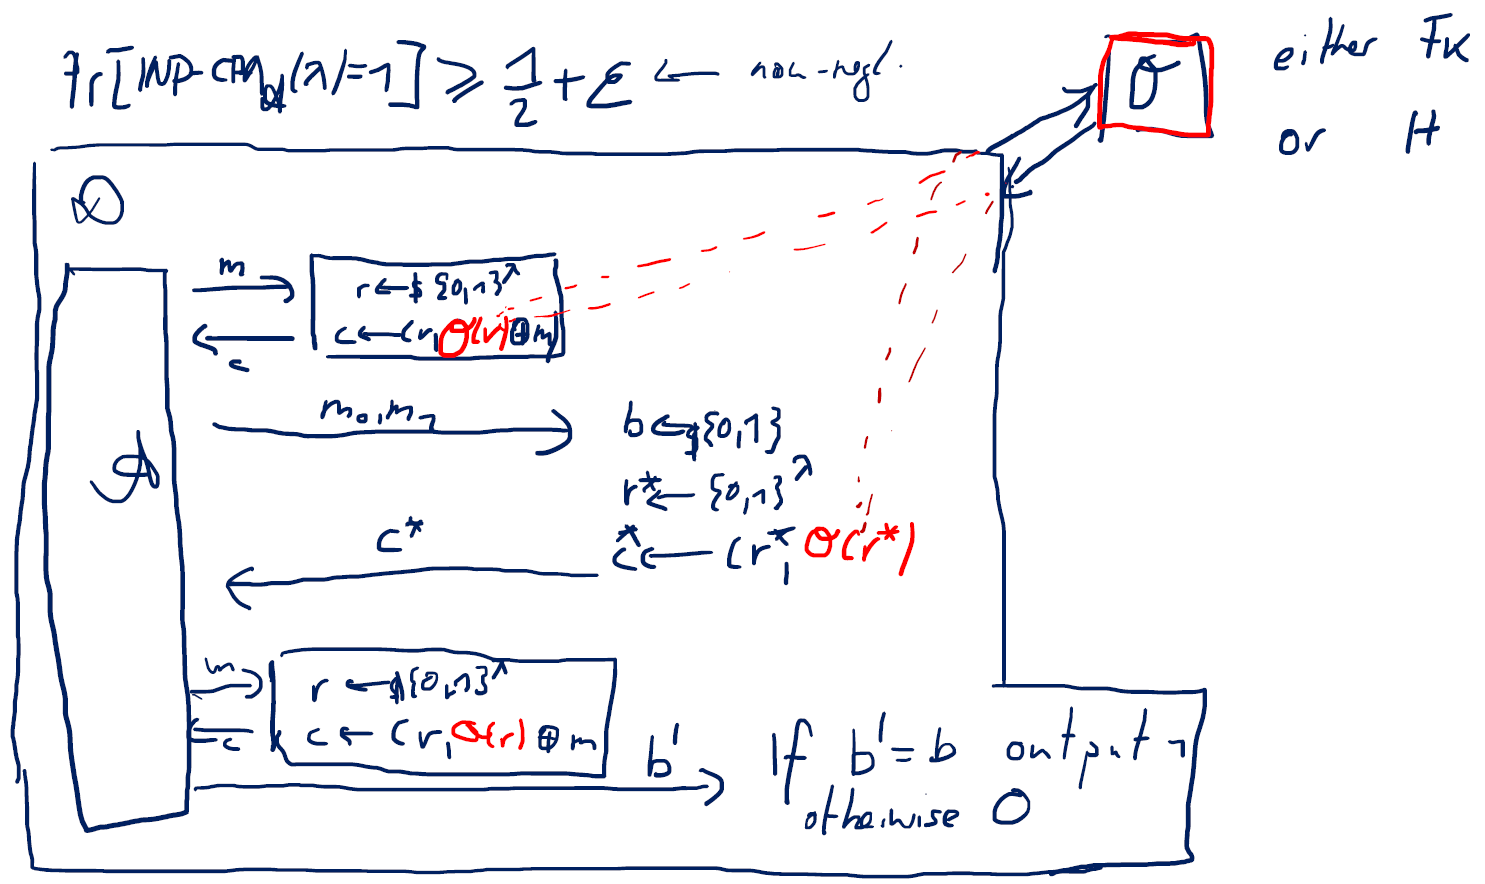
\includegraphics[width=148mm]{Graphics/CPA/cpa5.png}
		\end{center}
		\underline{Case distinction:}
		\begin{enumerate}
			\item If $\mathcal{O} = F_K$ then $\mathcal{D}$ simulates $IND-CPA_{\mathcal{A}}(\lambda)$ experiment:
				$$Pr[\mathcal{D}^{F_K(\cdot)}(1^{\lambda}) = 1] = Pr[IND-CPA_{\mathcal{A}}(\lambda) = 1] \geq \frac{1}{2} + \epsilon$$
			\item If $\mathcal{O} = H$ then $\mathcal{D}$ simulates $IND-CPA'_{\mathcal{A}}(\lambda)$ experiment:
				$$Pr[\mathcal{D}^{H(\cdot)}(1^{\lambda}) = 1] = Pr[IND-CPA'_{\mathcal{A}}(\lambda) = 1] \leq \frac{1}{2} + \frac{q}{2^{\lambda}}$$
		\end{enumerate}
		Now we can follow
		$$Pr[\mathcal{D}^{F_K(\cdot)}(1^{\lambda}) = 1] - Pr[\mathcal{D}^{H(\cdot)}(1^{\lambda}) = 1]
		\geq \frac{1}{2} + \epsilon - \frac{1}{2} - \frac{q}{2^{\lambda}} = \epsilon - \frac{q}{2^{\lambda}}$$
		We know that $\epsilon$ is negligible and $\frac{q}{2^{\lambda}}$ is non-negligible, so it follows that the difference is not negligible! 
	\end{proof}
	
\section{Summary}
	\begin{itemize}
		\item Key reuse requires a stronger security notion: $IND-CPA$ security
		\item $IND-CPA$ secure encryption schemes cannot be deterministic!
		\item $IND-CPA$ secure encryption can be constructed from pseudorandom functions (PRFs)
	\end{itemize}




































